\section{Misura $e/m$}
	Per effettuare  la misura del rapporto e/m
	si inserisce il bulbo nell'alloggiamonto posto tra le bobine.
	Attraverso il dispositivo di alimentazione si è fornito 
	al filamento interno ,una corrente alternata sufficiente alla produzione di \e 
	per effetto termoionico;tale corrente corrisponde a
	$V_{heat}\geqq$\SI{3 }{\volt}\footnote{valore nominale}.
	Sempre attraverso il dispositivo di alimentazione si è fornita una 
	d.d.p. accelerante $V_{acc}\geqq$\SI{150 \pm 1}{\volt}.
	
	In assenza di campo magnetico si osserva che il pennellino luminoso ,
	dovuto al moto degli \e, risulta essere lineare.
	\bigskip
	$$nelle- nostre- foto- non- c'è -ditemi- voi -ne- so- na- di- n- grppo [ma-di-qesto-anno]$$
	\bigskip
	
	Si è adesso alimentato le bobine di Halmotz con una tensione $V_{coil}=$\SI{7.5 \pm 0.1}{\volt}\footnote[1]{}  
	avendo qindi na corrente di $I_{coil}=$\SI{0.96 \pm 1}{\ampere}\footnote[1]{}.
	Si osserva che in presenza di $B_z$ il pennellino elettronico descrive n orbita 
	circolare.
	
	Per i valori di $V_{coil}$ e $V_{acc}$ appena fissati si è  osservata la variazione del pennellino elettronico al variare di 	$V_{heat}$.
	Per valori di $V_{heat}<$\SI{3}{\volt}
	non si osserva emissione di \e; ciò suggerisce la presenza di un valore di soglia
	$\sim 3 V$. Per valori $V_{heat}>$\SI{3}{\volt} ma ad esso prossimo
	si osserva che il fascio sia meno definito rispetto alle tensioni superiori;
	qesto effetto rislta compatibile col fatto che il filamento si trovi ,o termalizzi, a temperatre più basse qindi emetta meno \e;
	si osserva inoltre che per tali valori il pennellino elettronico si presenta 
	doppio.
	
	Fissato $V_{heat}=$\SI{6}{\volt}\footnote{valore nominale} si è campionato,attraverso l'acqisizione di varie foto,il moto degli \e al variare di $V_{coil}$, consegentemente di $I_{coil}$, e di $V_{acc}$.
	\begin{table}[hb]
		\centering
		\begin{tabular}{|c|c|c|c|}
			\toprule
			n foto & 	$V_{acc}$  & 	$V_{coil}$ & $I_{coil}$ \\
			\midrule
			5 & \SI{200 \pm 1}{\volt} &\SI{6.0 \pm 0.1}{\volt} & \SI{0.77 \pm 0.01}{\ampere}\\
			6 & \SI{200 \pm 1}{\volt} &\SI{6.3 \pm 0.1}{\volt} & \SI{0.80 \pm 0.01}{\ampere}\\
			7 & \SI{200 \pm 1}{\volt} &\SI{6.6 \pm 0.1}{\volt} & \SI{0.84 \pm 0.01}{\ampere}\\
			8 & \SI{200 \pm 1}{\volt} &\SI{6.9 \pm 0.1}{\volt} & \SI{0.87 \pm 0.01}{\ampere}\\
			9 & \SI{200 \pm 1}{\volt} &\SI{7.2 \pm 0.1}{\volt} & \SI{0.92 \pm 0.01}{\ampere}\\
			10 & \SI{200 \pm 1}{\volt} &\SI{7.5 \pm 0.1}{\volt} & \SI{0.96 \pm 0.01}{\ampere}\\
			11 & \SI{200 \pm 1}{\volt} &\SI{7.8 \pm 0.1}{\volt} & \SI{0.99 \pm 0.01}{\ampere}\\
			12 & \SI{200 \pm 1}{\volt} &\SI{8.1 \pm 0.1}{\volt} & \SI{1.03 \pm 0.01}{\ampere}\\
			13 & \SI{200 \pm 1}{\volt} &\SI{8.4 \pm 0.1}{\volt} & \SI{1.07 \pm 0.01}{\ampere}\\
			14 & \SI{200 \pm 1}{\volt} &\SI{8.7 \pm 0.1}{\volt} & \SI{1.10 \pm 0.01}{\ampere}\\
			15 & \SI{200 \pm 1}{\volt} &\SI{9.0 \pm 0.1}{\volt} & \SI{1.15 \pm 0.01}{\ampere}\\
			16 & \SI{219 \pm 1}{\volt} &\SI{6.0 \pm 0.1}{\volt} & \SI{0.77 \pm 0.01}{\ampere}\\
			17 & \SI{219 \pm 1}{\volt} &\SI{6.3 \pm 0.1}{\volt} & \SI{0.80 \pm 0.01}{\ampere}\\
			18 & \SI{219 \pm 1}{\volt} &\SI{6.6 \pm 0.1}{\volt} & \SI{0.84 \pm 0.01}{\ampere}\\
			19 & \SI{219 \pm 1}{\volt} &\SI{6.9 \pm 0.1}{\volt} & \SI{0.87 \pm 0.01}{\ampere}\\
			20 & \SI{219 \pm 1}{\volt} &\SI{7.2 \pm 0.1}{\volt} & \SI{0.92 \pm 0.01}{\ampere}\\
			21 & \SI{219 \pm 1}{\volt} &\SI{7.5 \pm 0.1}{\volt} & \SI{0.96 \pm 0.01}{\ampere}\\
			22 & \SI{219 \pm 1}{\volt} &\SI{7.8 \pm 0.1}{\volt} & \SI{0.99 \pm 0.01}{\ampere}\\
			23 & \SI{219 \pm 1}{\volt} &\SI{8.1 \pm 0.1}{\volt} & \SI{1.03 \pm 0.01}{\ampere}\\
			24 & \SI{219 \pm 1}{\volt} &\SI{8.4 \pm 0.1}{\volt} & \SI{1.07 \pm 0.01}{\ampere}\\
			25 & \SI{219 \pm 1}{\volt} &\SI{8.7 \pm 0.1}{\volt} & \SI{1.10 \pm 0.01}{\ampere}\\
			26 & \SI{219 \pm 1}{\volt} &\SI{9.0 \pm 0.1}{\volt} & \SI{1.15 \pm 0.01}{\ampere}\\
			27 & \SI{239 \pm 1}{\volt} &\SI{6.0 \pm 0.1}{\volt} & \SI{0.77 \pm 0.01}{\ampere}\\
			28 & \SI{239 \pm 1}{\volt} &\SI{6.3 \pm 0.1}{\volt} & \SI{0.80 \pm 0.01}{\ampere}\\
			29 & \SI{239 \pm 1}{\volt} &\SI{6.6 \pm 0.1}{\volt} & \SI{0.84 \pm 0.01}{\ampere}\\
			30 & \SI{239 \pm 1}{\volt} &\SI{6.9 \pm 0.1}{\volt} & \SI{0.87 \pm 0.01}{\ampere}\\
			31 & \SI{239 \pm 1}{\volt} &\SI{7.2 \pm 0.1}{\volt} & \SI{0.92 \pm 0.01}{\ampere}\\
			32 & \SI{239 \pm 1}{\volt} &\SI{7.5 \pm 0.1}{\volt} & \SI{0.96 \pm 0.01}{\ampere}\\
			33 & \SI{239 \pm 1}{\volt} &\SI{7.8 \pm 0.1}{\volt} & \SI{0.99 \pm 0.01}{\ampere}\\
			34 & \SI{239 \pm 1}{\volt} &\SI{8.1 \pm 0.1}{\volt} & \SI{1.03 \pm 0.01}{\ampere}\\
			35 & \SI{239 \pm 1}{\volt} &\SI{8.4 \pm 0.1}{\volt} & \SI{1.07 \pm 0.01}{\ampere}\\
			36 & \SI{239 \pm 1}{\volt} &\SI{8.7 \pm 0.1}{\volt} & \SI{1.10 \pm 0.01}{\ampere}\\
			37 & \SI{239 \pm 1}{\volt} &\SI{9.0 \pm 0.1}{\volt} & \SI{1.15 \pm 0.01}{\ampere}\\
			38 & \SI{261 \pm 1}{\volt} &\SI{6.0 \pm 0.1}{\volt} & \SI{0.77 \pm 0.01}{\ampere}\\
			39 & \SI{261 \pm 1}{\volt} &\SI{6.3 \pm 0.1}{\volt} & \SI{0.80 \pm 0.01}{\ampere}\\
			40 & \SI{261 \pm 1}{\volt} &\SI{6.6 \pm 0.1}{\volt} & \SI{0.84 \pm 0.01}{\ampere}\\
			41 & \SI{261 \pm 1}{\volt} &\SI{6.9 \pm 0.1}{\volt} & \SI{0.87 \pm 0.01}{\ampere}\\
			42 & \SI{261 \pm 1}{\volt} &\SI{7.2 \pm 0.1}{\volt} & \SI{0.92 \pm 0.01}{\ampere}\\
			43 & \SI{261 \pm 1}{\volt} &\SI{7.5 \pm 0.1}{\volt} & \SI{0.96 \pm 0.01}{\ampere}\\
			44 & \SI{261 \pm 1}{\volt} &\SI{7.9 \pm 0.1}{\volt} & \SI{1.01 \pm 0.01}{\ampere}\\
			45 & \SI{261 \pm 1}{\volt} &\SI{8.1 \pm 0.1}{\volt} & \SI{1.03 \pm 0.01}{\ampere}\\
			46 & \SI{261 \pm 1}{\volt} &\SI{8.4 \pm 0.1}{\volt} & \SI{1.07 \pm 0.01}{\ampere}\\
			47 & \SI{261 \pm 1}{\volt} &\SI{8.7 \pm 0.1}{\volt} & \SI{1.10 \pm 0.01}{\ampere}\\
			48 & \SI{261 \pm 1}{\volt} &\SI{9.0 \pm 0.1}{\volt} & \SI{1.14 \pm 0.01}{\ampere}\\
			49 & \SI{282 \pm 1}{\volt} &\SI{6.0 \pm 0.1}{\volt} & \SI{0.76 \pm 0.01}{\ampere}\\
			50 & \SI{282 \pm 1}{\volt} &\SI{6.3 \pm 0.1}{\volt} & \SI{0.80 \pm 0.01}{\ampere}\\
			51 & \SI{282 \pm 1}{\volt} &\SI{6.6 \pm 0.1}{\volt} & \SI{0.84 \pm 0.01}{\ampere}\\
			52 & \SI{282 \pm 1}{\volt} &\SI{6.9 \pm 0.1}{\volt} & \SI{0.87 \pm 0.01}{\ampere}\\
			53 & \SI{282 \pm 1}{\volt} &\SI{7.2 \pm 0.1}{\volt} & \SI{0.92 \pm 0.01}{\ampere}\\
			54 & \SI{282 \pm 1}{\volt} &\SI{7.5 \pm 0.1}{\volt} & \SI{0.95 \pm 0.01}{\ampere}\\
			55 & \SI{282 \pm 1}{\volt} &\SI{7.8 \pm 0.1}{\volt} & \SI{0.99 \pm 0.01}{\ampere}\\
			56 & \SI{282 \pm 1}{\volt} &\SI{8.1 \pm 0.1}{\volt} & \SI{1.03 \pm 0.01}{\ampere}\\
			57 & \SI{282 \pm 1}{\volt} &\SI{8.4 \pm 0.1}{\volt} & \SI{1.07 \pm 0.01}{\ampere}\\
			58 & \SI{282 \pm 1}{\volt} &\SI{8.7 \pm 0.1}{\volt} & \SI{1.10 \pm 0.01}{\ampere}\\
			59 & \SI{282 \pm 1}{\volt} &\SI{9.0 \pm 0.1}{\volt} & \SI{1.15 \pm 0.01}{\ampere}\\
			60 & \SI{302 \pm 1}{\volt} &\SI{6.0 \pm 0.1}{\volt} & \SI{0.76 \pm 0.01}{\ampere}\\
			61 & \SI{302 \pm 1}{\volt} &\SI{6.3 \pm 0.1}{\volt} & \SI{0.80 \pm 0.01}{\ampere}\\
			62 & \SI{302 \pm 1}{\volt} &\SI{6.6 \pm 0.1}{\volt} & \SI{0.84 \pm 0.01}{\ampere}\\
			63 & \SI{302 \pm 1}{\volt} &\SI{6.9 \pm 0.1}{\volt} & \SI{0.88 \pm 0.01}{\ampere}\\
			64 & \SI{302 \pm 1}{\volt} &\SI{7.2 \pm 0.1}{\volt} & \SI{0.91 \pm 0.01}{\ampere}\\
			65 & \SI{302 \pm 1}{\volt} &\SI{7.5 \pm 0.1}{\volt} & \SI{0.95 \pm 0.01}{\ampere}\\
			66 & \SI{302 \pm 1}{\volt} &\SI{7.8 \pm 0.1}{\volt} & \SI{0.99 \pm 0.01}{\ampere}\\
			67 & \SI{302 \pm 1}{\volt} &\SI{8.1 \pm 0.1}{\volt} & \SI{1.03 \pm 0.01}{\ampere}\\
			68 & \SI{302 \pm 1}{\volt} &\SI{8.4 \pm 0.1}{\volt} & \SI{1.07 \pm 0.01}{\ampere}\\
			69 & \SI{302 \pm 1}{\volt} &\SI{8.7 \pm 0.1}{\volt} & \SI{1.10 \pm 0.01}{\ampere}\\
			70 & \SI{302 \pm 1}{\volt} &\SI{9.0 \pm 0.1}{\volt} & \SI{1.15 \pm 0.01}{\ampere}\\
			\bottomrule
		\end{tabular}
		\caption{Si riportano i valori corrispondenti alle nostre acqisizioni.I set dal 1 al 4 sono stati impiegati per cercare le impostazioni ottimali della fotocamera.}
		\label{t:b}
	\end{table}
	 si riportano i valori corrispondenti alle acqisizioni in \tablename{ \ref{t:b}}.

	
	
	
	
	Si riportano a scopo illustrativo alcune delle acquisizioni
		\begin{figure}[hb]
		\centering
		\subfloat[acquisizione n.11]{
			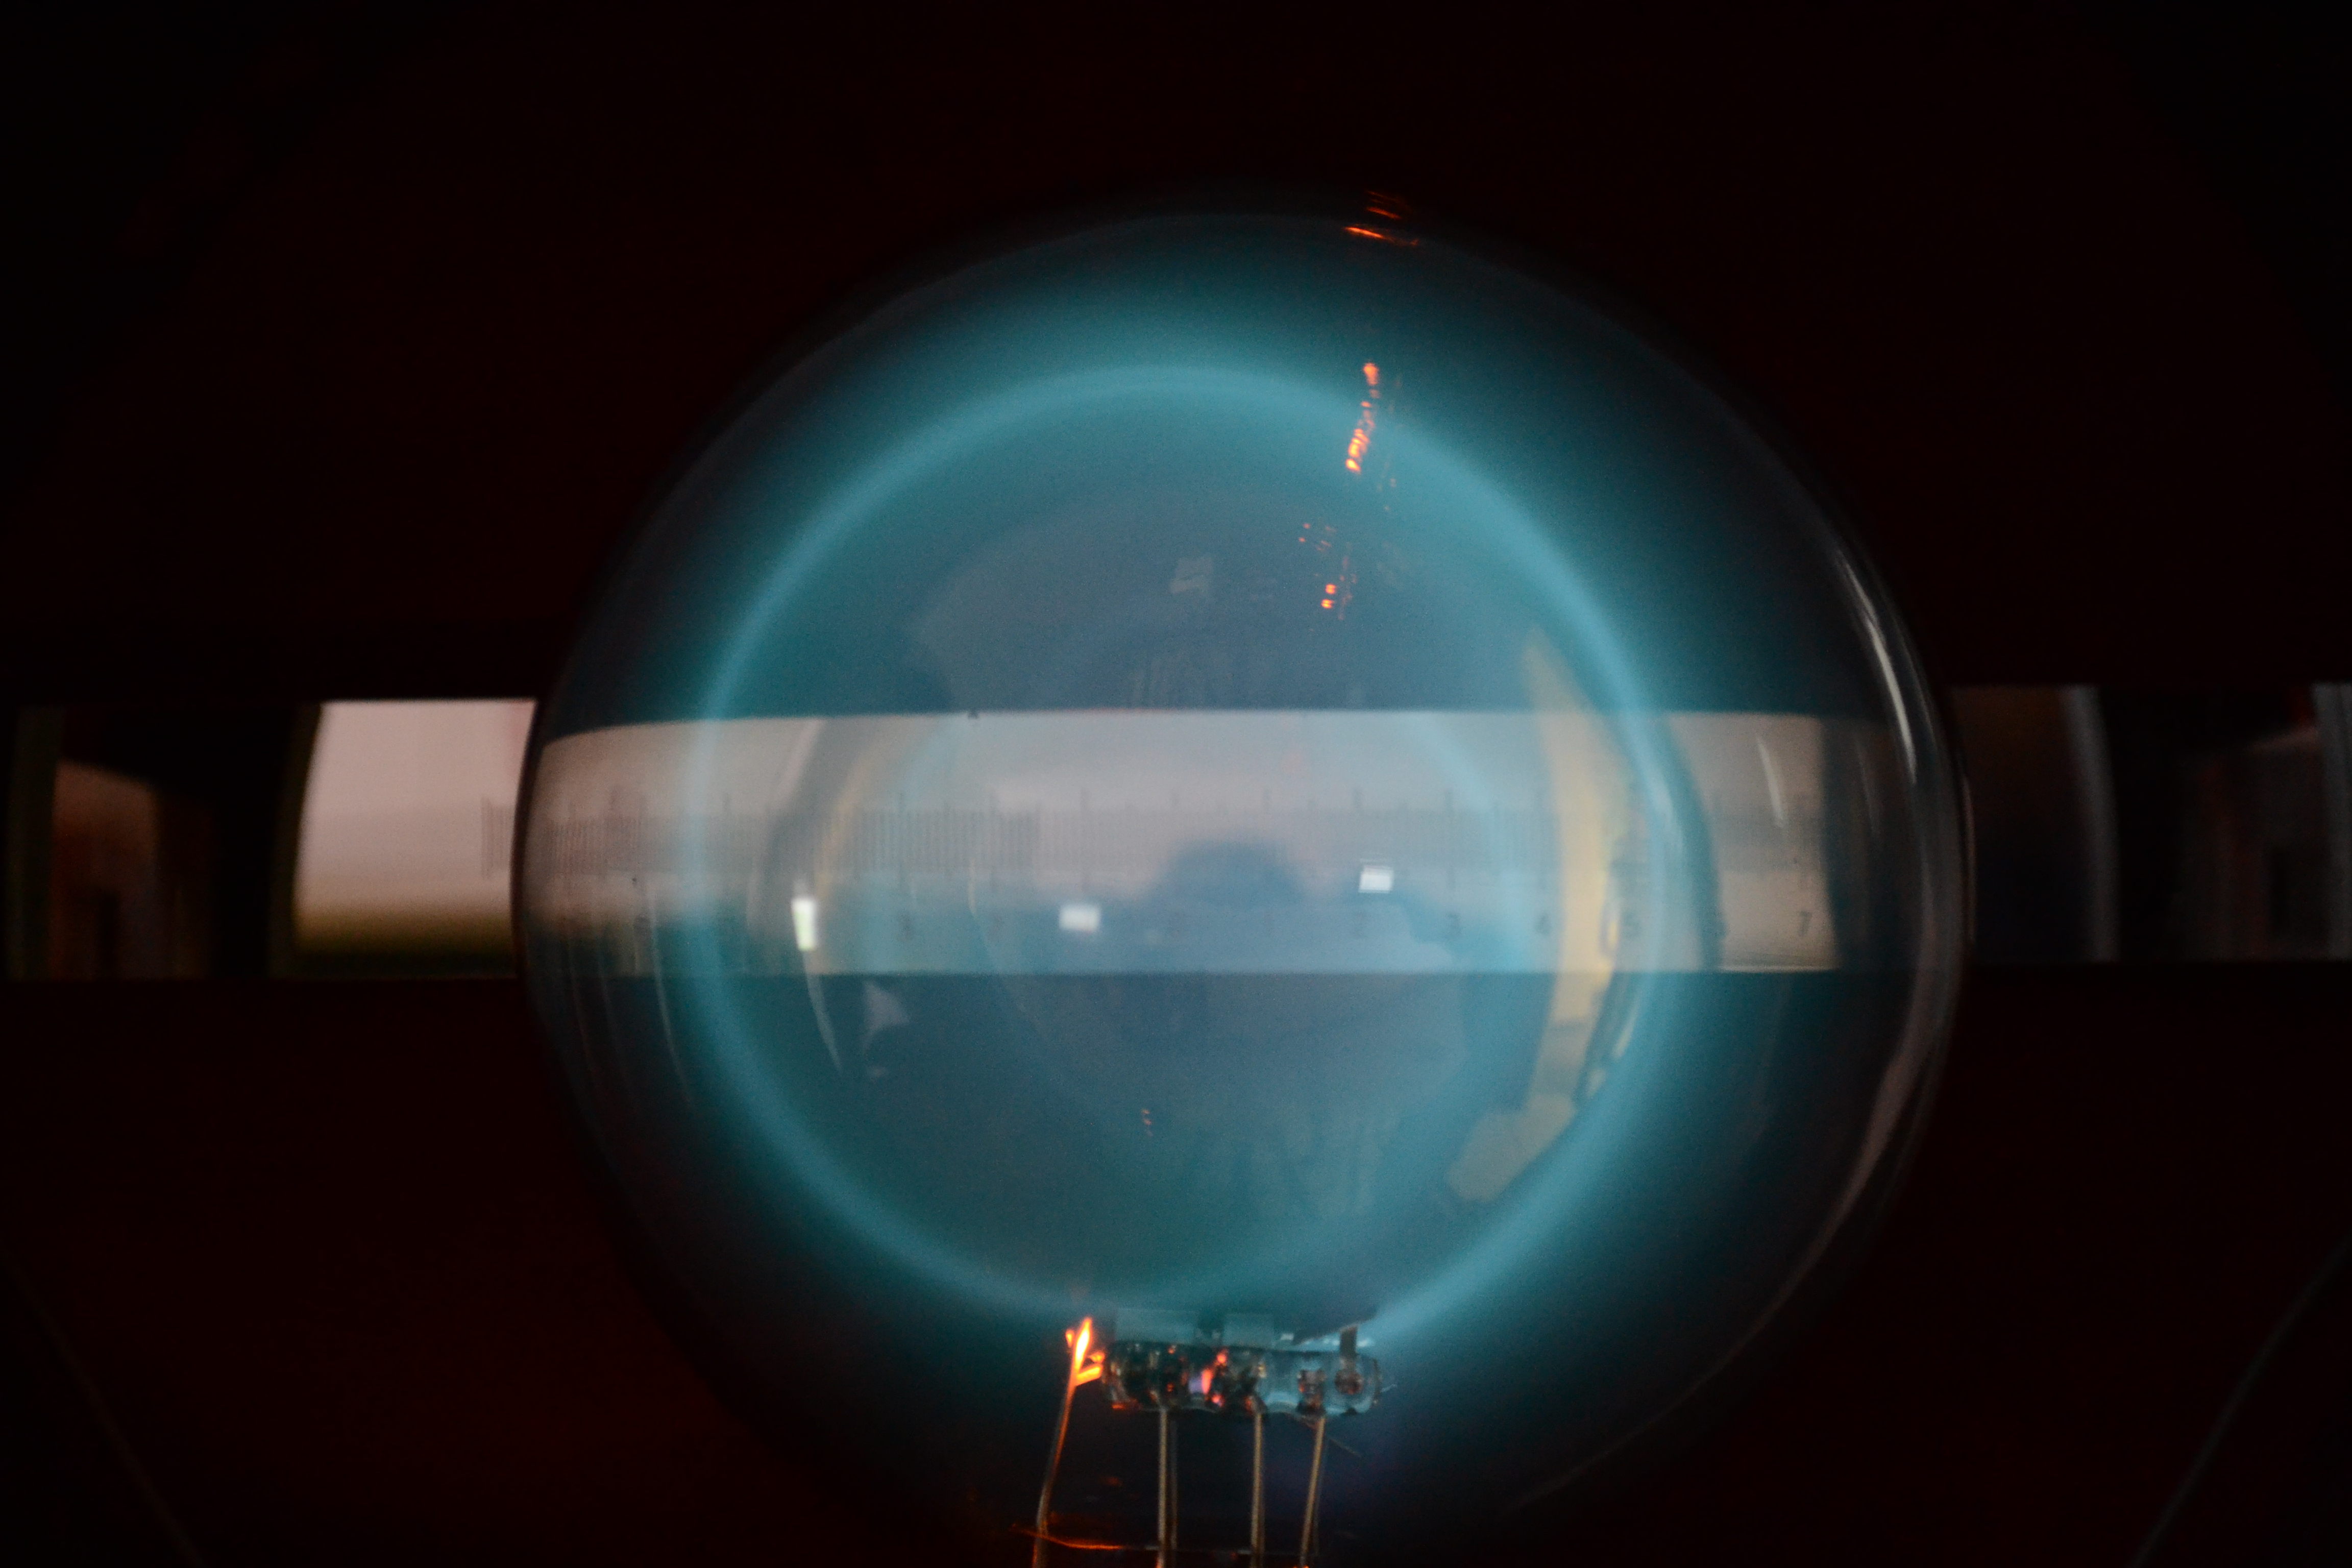
\includegraphics[scale=0.25]{./fig/(11).JPG}
			\label{f:acquisizione-fiev}
			}
		\subfloat[acquisizione n.22]{
			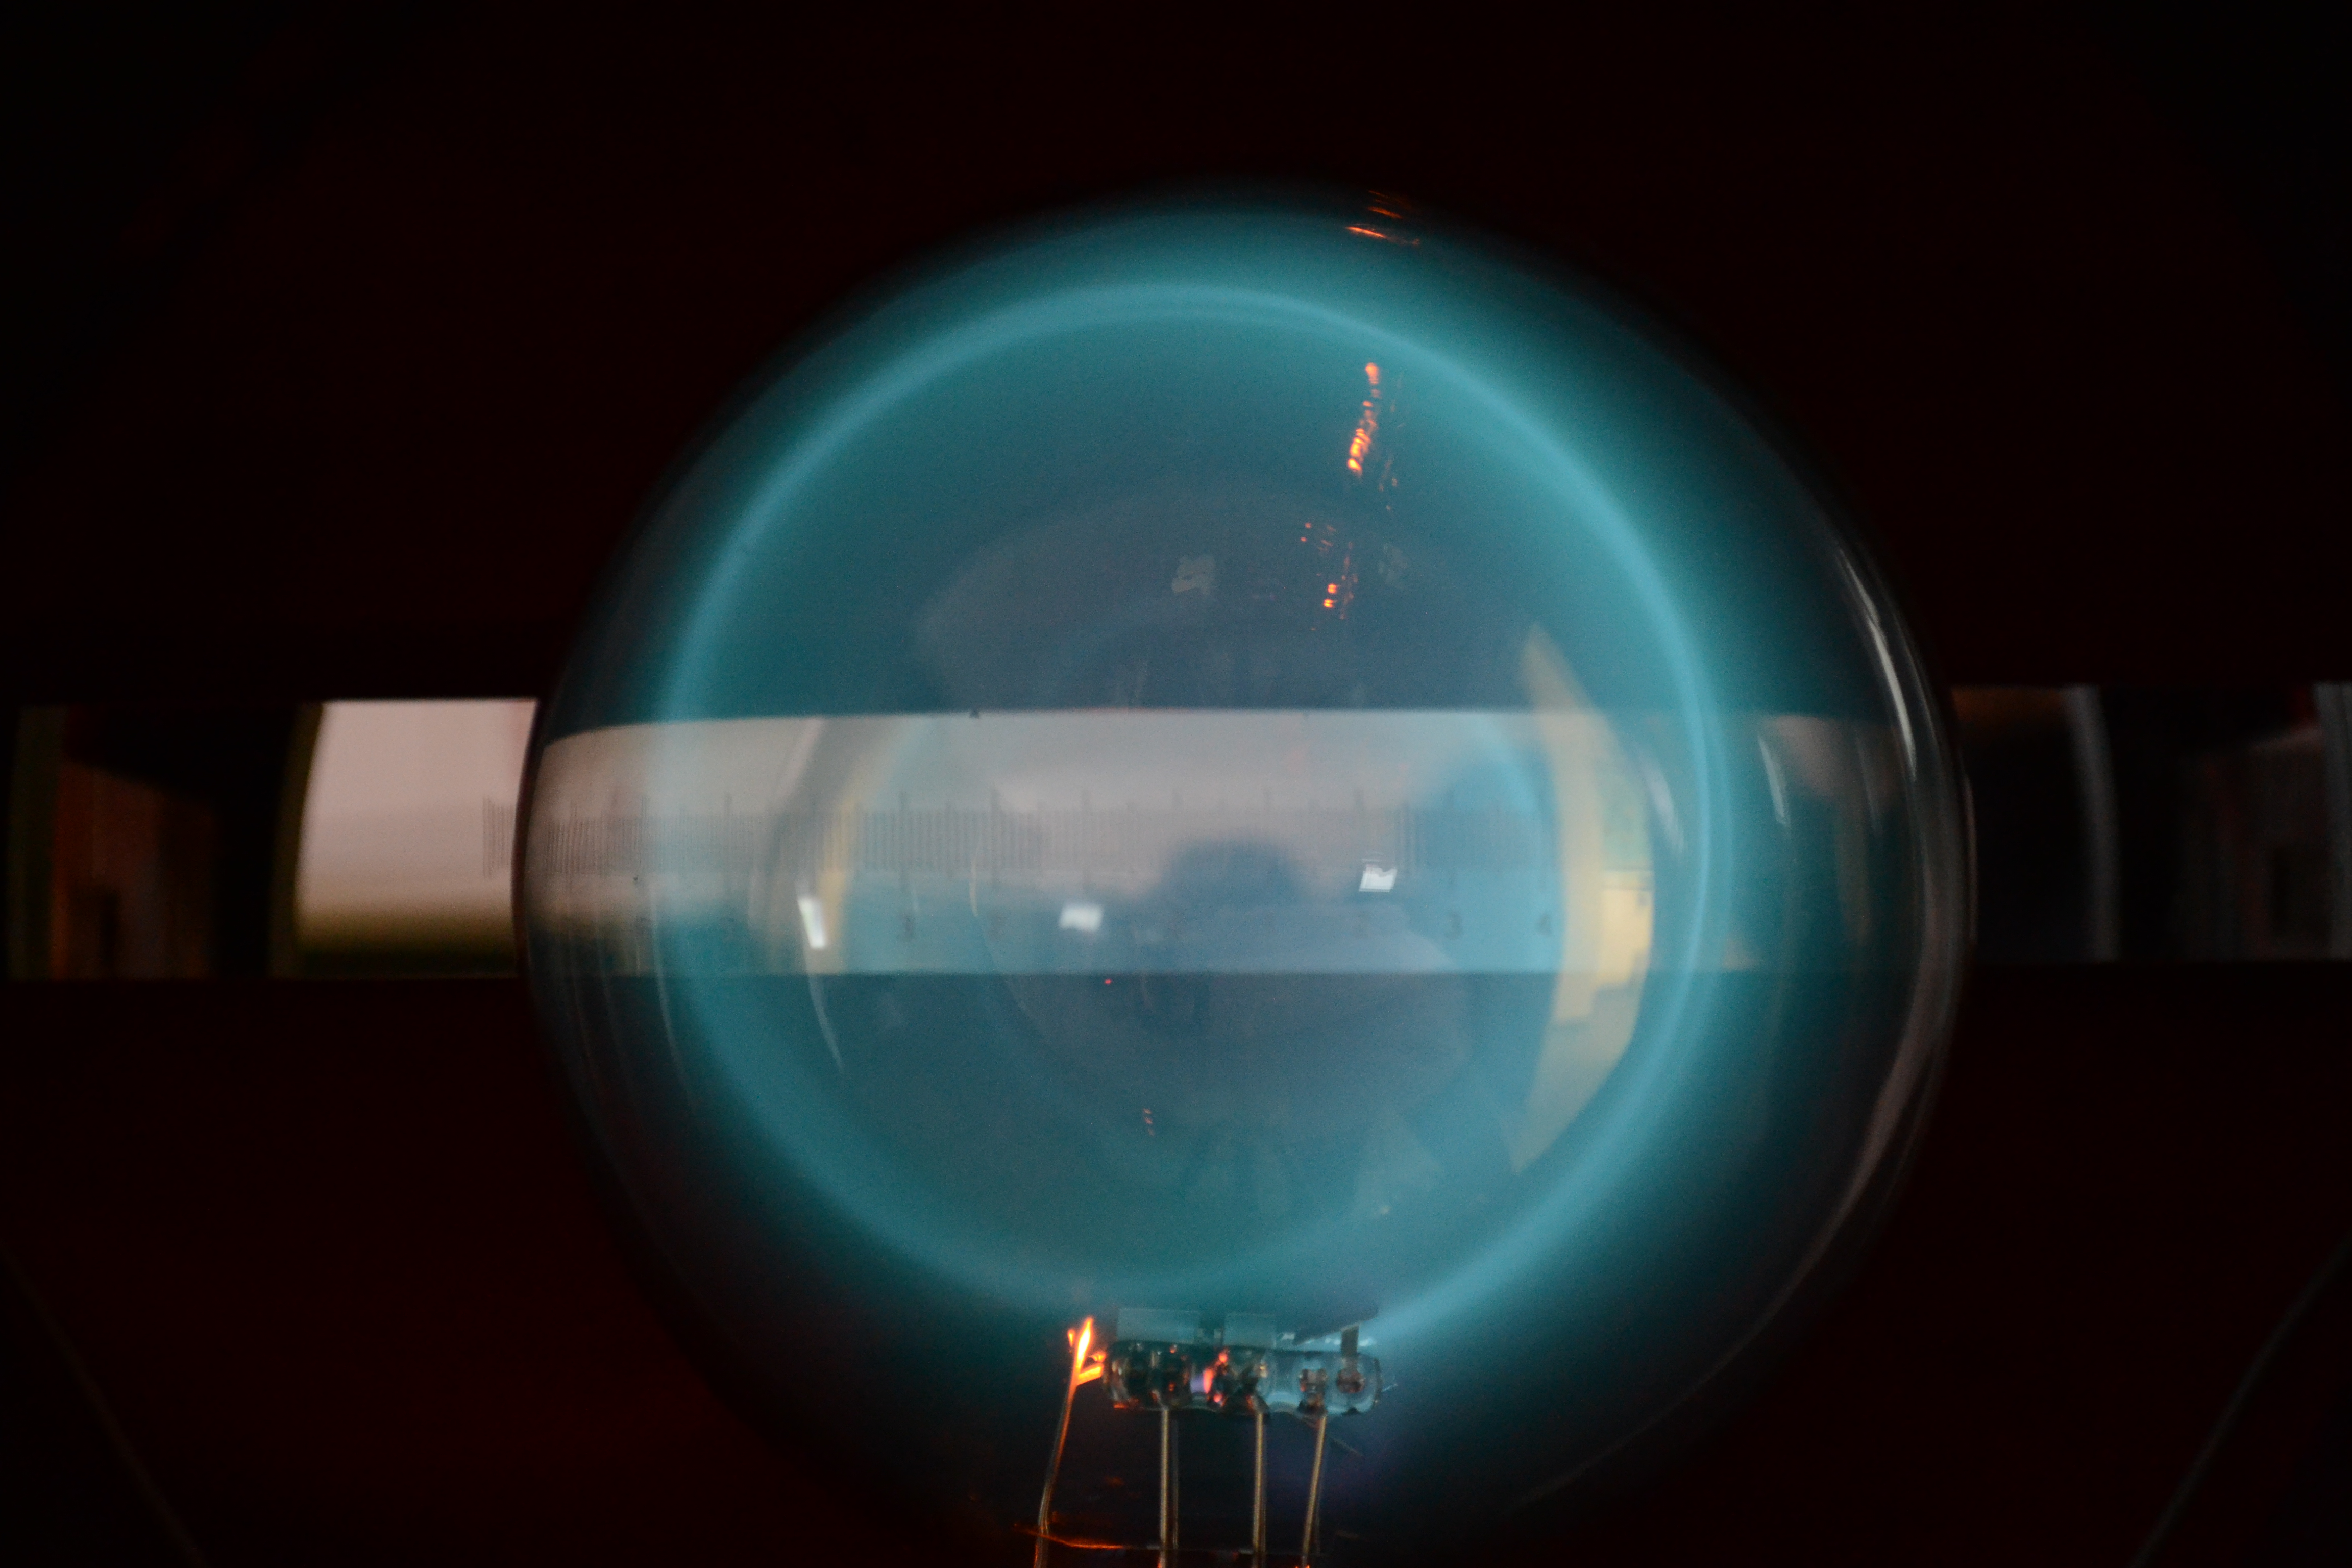
\includegraphics[scale=0.25]{./fig/(22).JPG}
			}\\
		\subfloat[acquisizione n.44]{
			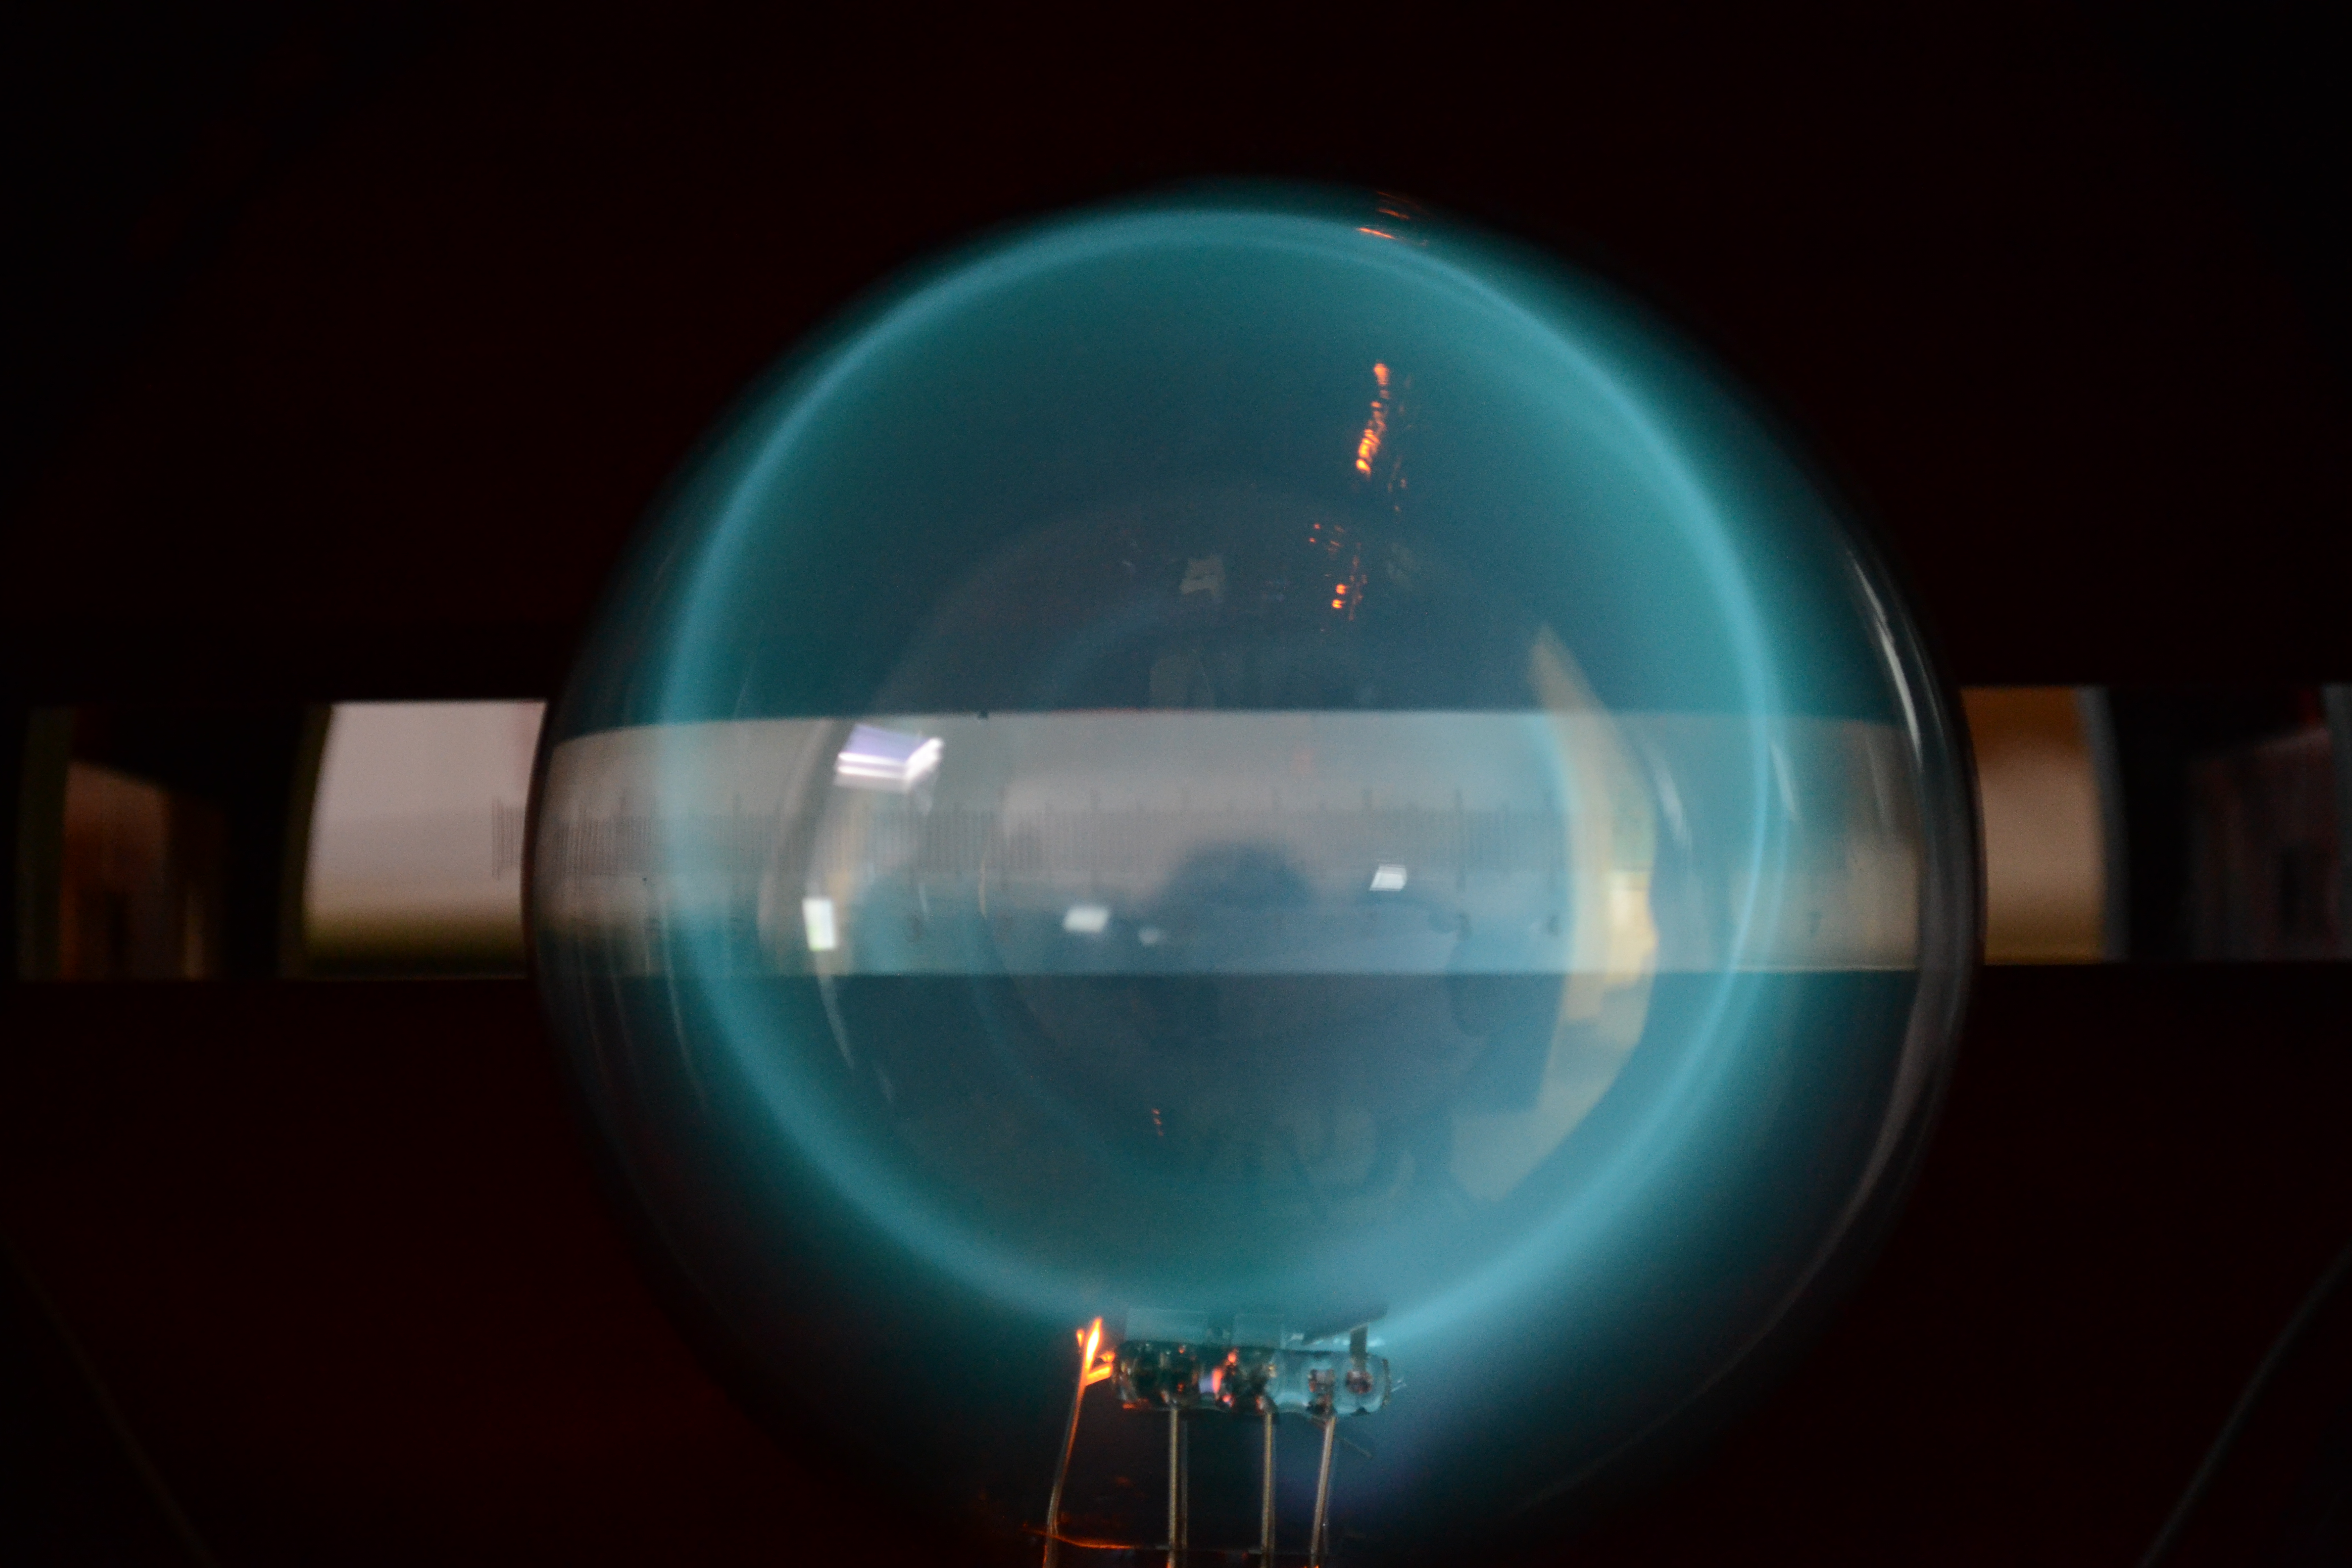
\includegraphics[scale=0.25]{./fig/(44).JPG}
		}
		\subfloat[acquisizione n.58]{
			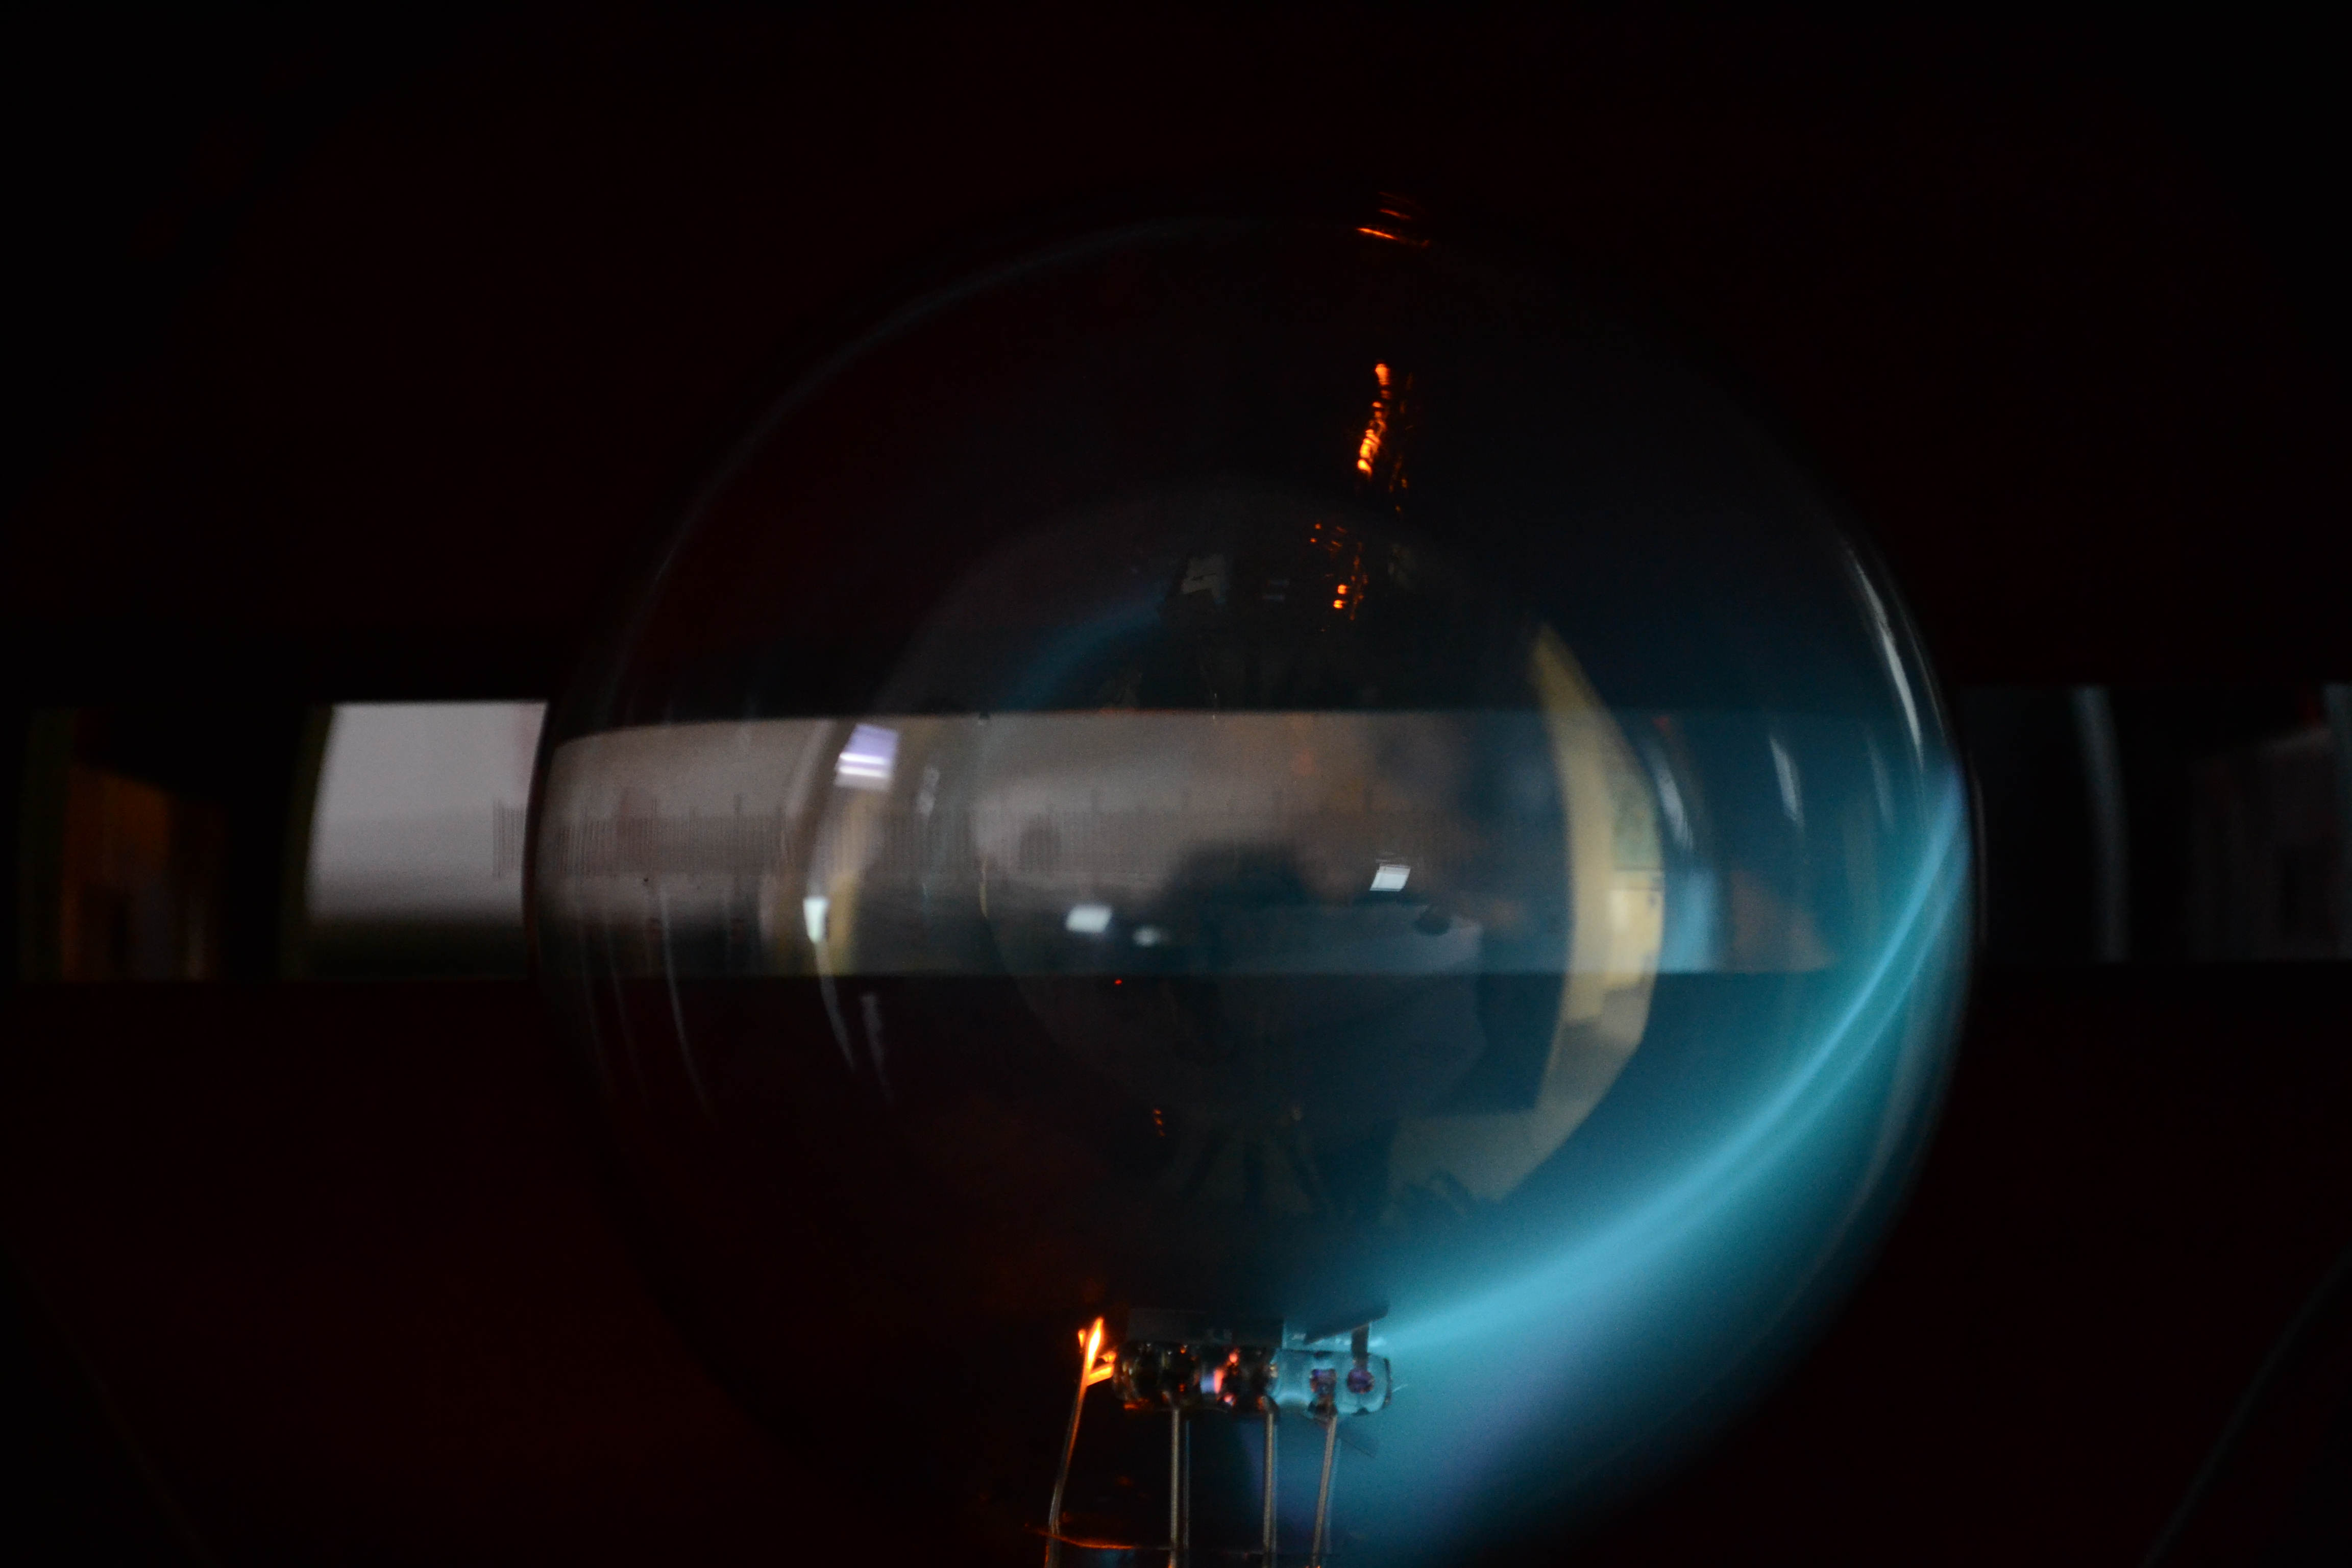
\includegraphics[scale=0.25]{./fig/(58).JPG}
				\label{f:acquisizione-inter}
		}
		\caption{esempio delle acquisizioni effettuate.Si segnala che per alcuni valori del compo accelerante si osserva un affievolirsi della traccia sul tratto terminale della circonferenza (\figurename{ \ref{f:acquisizione-fiev}}); ciò è dovuto alla diminuzione di \e di energia sufficiente per l'eccitazione del gas contenuto nel bulbo.
		Per taluni settaggi di $V_{acc}$ e $I_{coil}$ il raggio di curvatura risulta essere maggiore della regione del bulbo,pertanto la traccia si interrompe alla frontiera del bulbo(\figurename{ \ref{f:acquisizione-inter}}).
		Per le acquisizioni qualora la traccia risultasse troppo fievole per essere letta o non presentasse un orbita completa si sono impiegati i punti corrispondenti alla traccia leggibile.
		}
		\label{f:acquisizione}
	\end{figure}
	
	
	
	
	
	
	
	 	 
	 
	In questa fase si è ritento effettare una stima al prim'ordine del rapporto e/m
	per controllare la validità della approsimazioni operative fatte sin ora.
	Per effettare tale prima stima si è considerata l'acquisizione n.[21]. Avendo stimato dalla scala posta dietro la seconda bobina un raggio $r\sim 5.5 [cm]$ e dai corrispondenti valori in \tablename{ \ref{t:b}}.
	Essendo 
	\begin{equation}
	\frac{1}{2}m {v_e}^2=e V_{acc}
	\end{equation}\\
	 e per avere un moto circolare si deve ottenere una forza centripeta
	\begin{equation}
		F_c = \frac{m {v_e}^2}{r}= e v_e B_z
	\end{equation}
	si ottiene pertanto
	\begin{equation}
		\frac{e}{m}=\frac{v_e}{B_z r}
	\end{equation}\label{eq:e/m}
	corrispondente nella stima effettata ad un valore di $\frac{e}{m}\sim 2.5 \cdot 10^{11}$\si{\frac{\coulomb}{\kilogram} }.
	Che risulta compatibile con il valore atteso;
	pertanto sono state considerate valide le approssimazionei effettuate sin ora.
\subsection{analisi e misura effettiva di e/m} 
	Per effettuare una misura effettiva del rapporto $e/m$ dalle acqusizioni
	fatte precedentemente;
	si sono digitalizzate le stesse impiegando il programma \textbf{Plotdigitizer???}.
	$$scrivo-a-braccio-perché-non-so-se-qanto-detto-ha-fnzionato$$
	Per ognuna di tali digitalizzazioni sono stati acqisite le cordinate relative ai pixels corrispondenti  punti posti della 
	sulla traiettoria del moto degli \e.
	Si è poi per ogni acquisizione effettuato un fit circolare ottenendo l'$r$ associato.
	
	Per effettuare la conversione tra le cordinate in pixels in metri si sono impiegate le \figurename{ \ref{f:scala}} e  \figurename{ \ref{f:scalano}}
	ottenendo quindi una corrispondenza biunivoca tra le cordinate in pixels ed in centimetri.
	Si è inoltre dovuto tenere conto di eventali aberrazioni dovte alla natura grafica
	delle nostre acqisizioni.
	Per l'aberrazione introdotta dal bulbo si è
	$$in-template-fanno-n-fit-polinomiale-Xcordinate-con-blbo-Y-no-blbo-fit di fx-che -ne -dite?$$.
	Effettata tale correzione si è inoltre dovuto tenere conto del fatto che le immagini acquisite dalla fotocamera presentano una deformazione dovuta alla geometria proiettiva;
	si assume che tale effetto sia analogo a quello riportato in 
	\begin{figure}[hb]
		\centering
			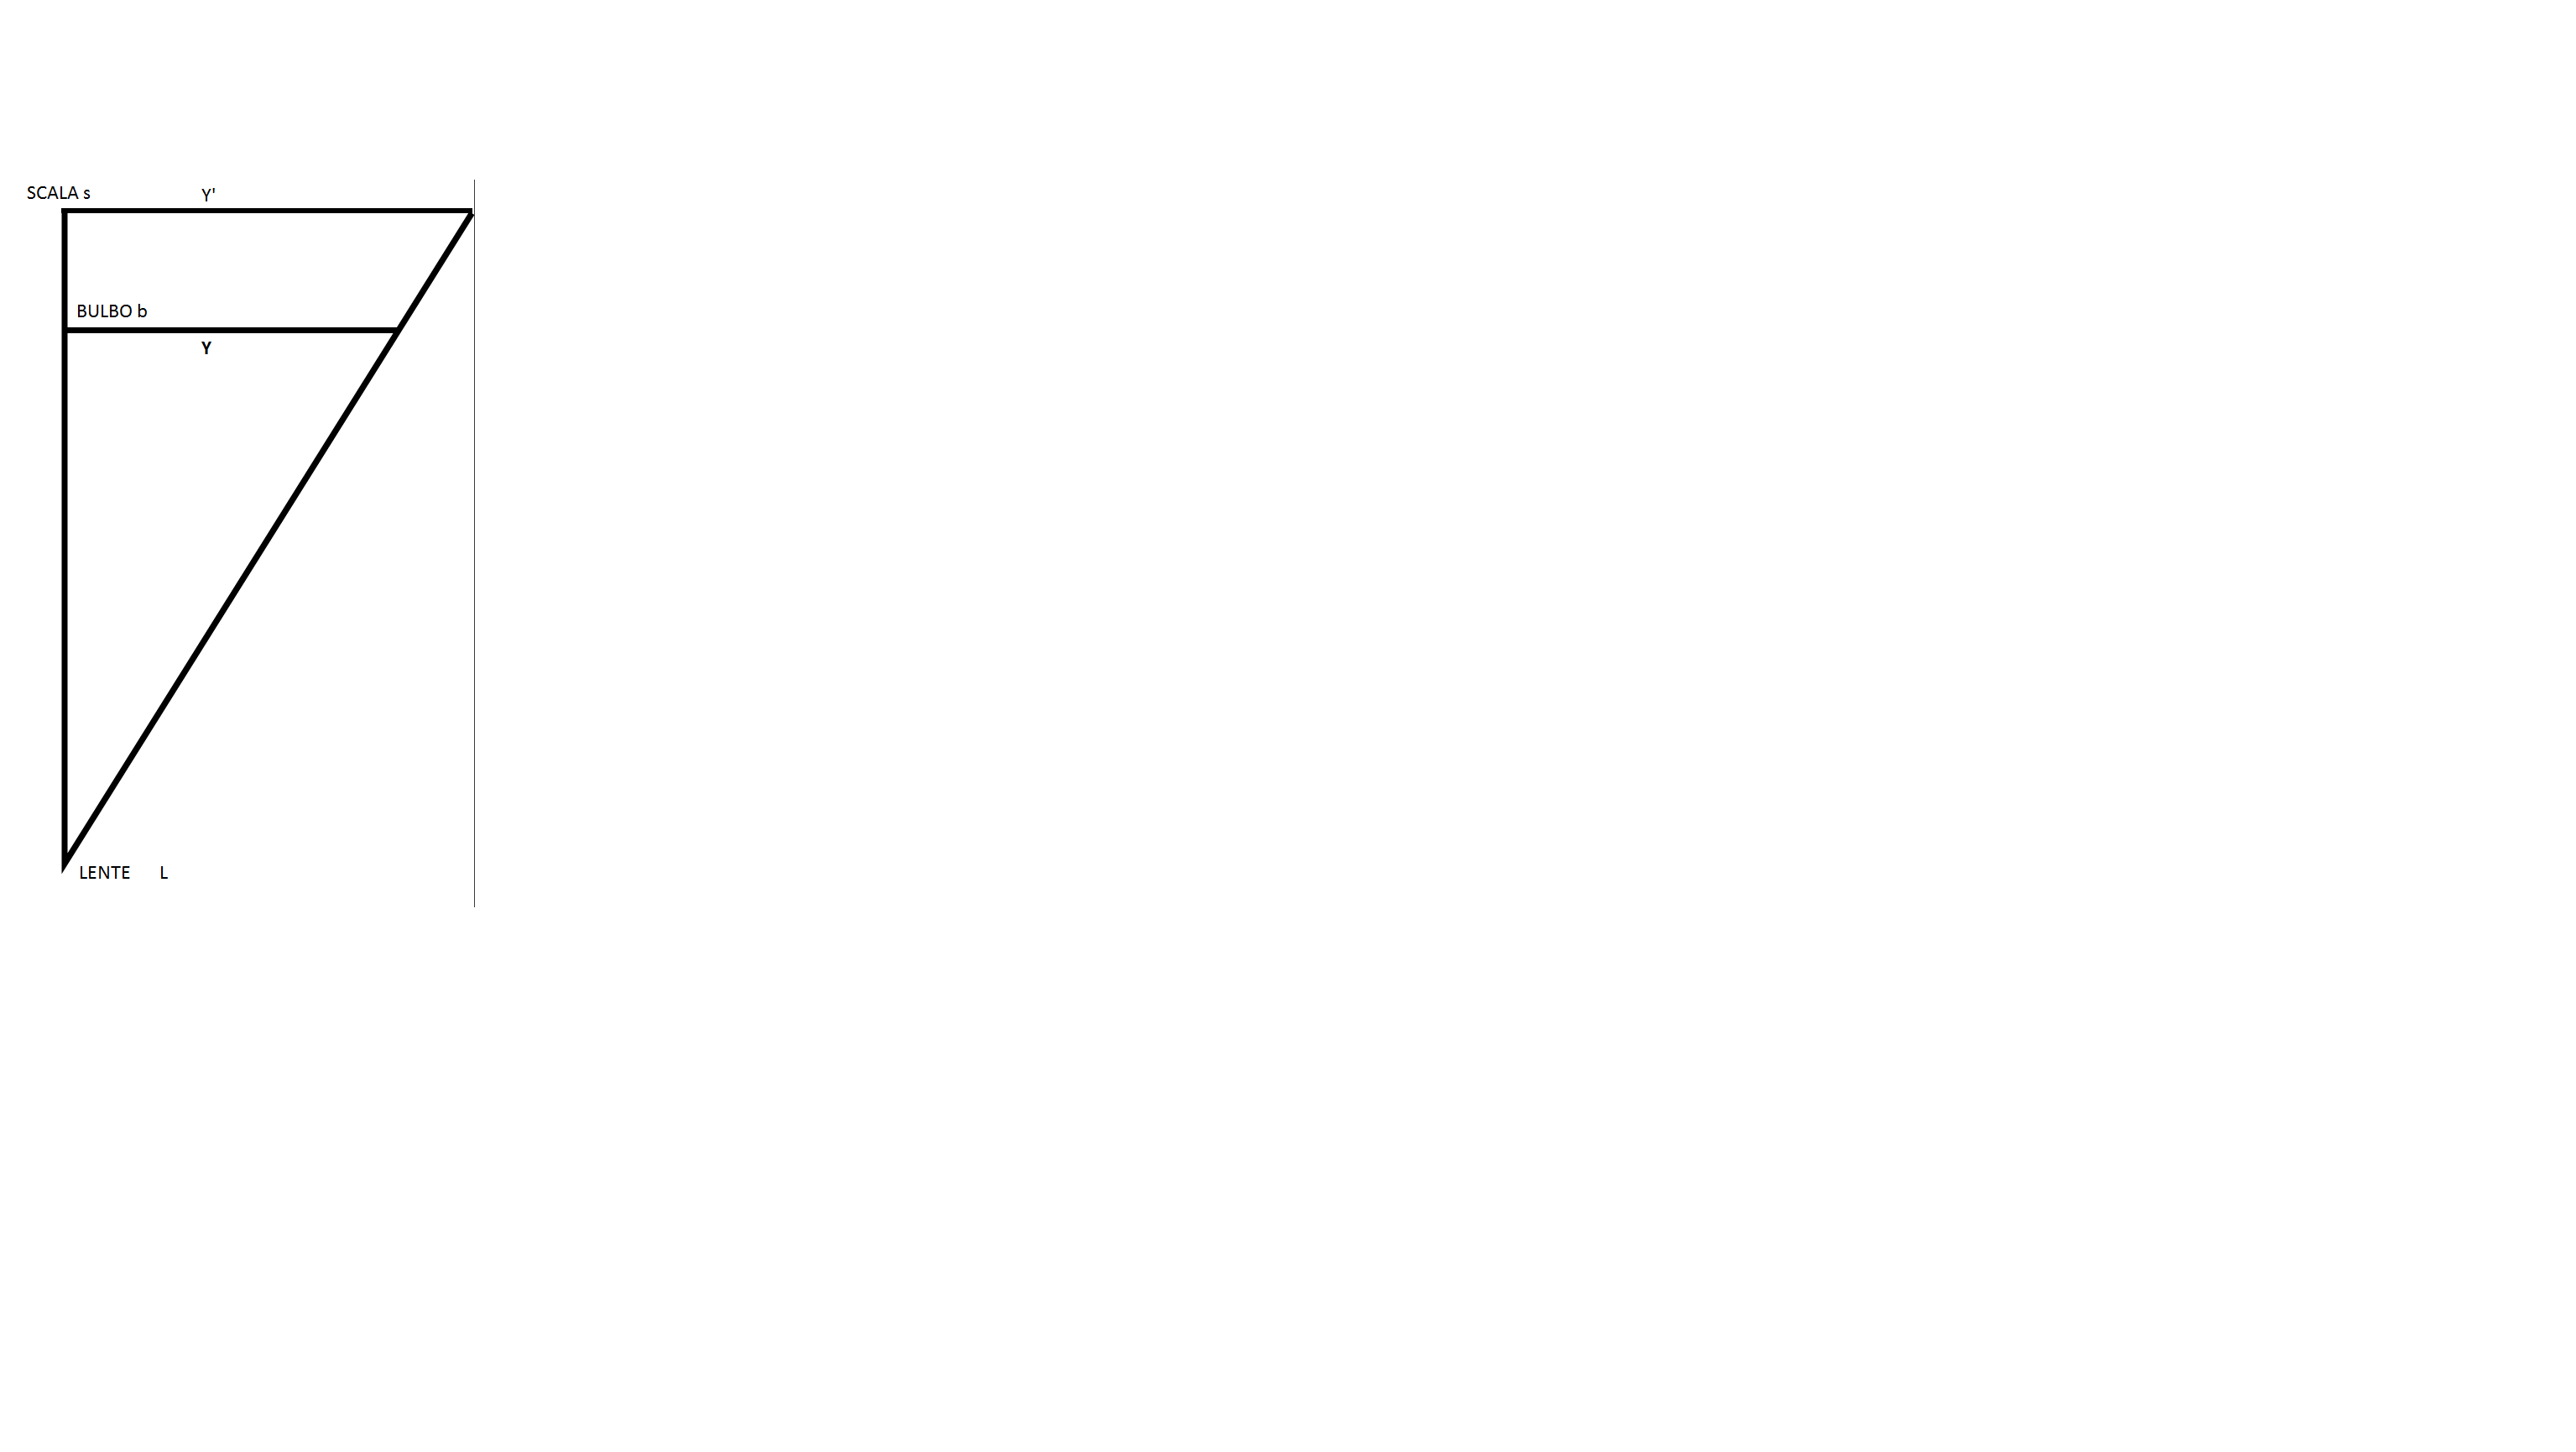
\includegraphics[scale=0.5]{./fig/geometria.png}
		
		\caption{immagine esplicativa dell'effetto di distorsione imputato alla geometria proiettiva.}
		\label{fig:geo-p}
		\end{figure}
	\figurename{ \ref{fig:geo-p}}.
	Per quantificare tale effetto si sono misurate la distanza lente della macchina 
	alla scala $ls=$\SI{56.8 \pm 0.1}{\cm}, e distanza lente bulbo  $lb=$\SI{45.8 \pm 0.2}{\cm}
	Essendo valida la relazione \begin{equation}
	Y=\frac{lb}{ls}\cdot Y^1 = a  Y^1
	\end{equation}\label{eq:geom}
	Ottenendo pertanto un coefficiente di correzione  $a=0.806 \pm 0.003$.
	Essendo quest'ultimo effetto sistematico sarà poi impiegato per correggere il rapporto e/m una volta ricavato.
	
	Effettuata la conversione pixels-cm e valutata l'aberrazione dovuta al bulbo 
	per i vari $r$ ottenti sulle varie acquisizioni, inpiegando l'\refeq{eq:e/m} e i relativi dati in \tablename{ \ref{t:b}} ottenendo per ogni set un rapporto ${e/m}_{n}$ ove n è il relativo numero di set.
	effettuando un fit di tali dati si ottiene il valore di $e/m$=\SI{0\pm 1000000}{\frac{\coulomb}{\kilogram}}  che risulta compatibile con il valore atteso di ${e/m}_{noto}=$
	\SI{1.75882002 e11}{\frac{\coulomb}{\kilogram}} $$da-controllare-e mettere- errore$$
	
%	Essendo lo spessore della traiettoria non ininfluente ,2-4 mm dipendentemente da quale acqusizione si stia analizzando, ad ognuno dei punti ottenuti
%	si è associata un incertezza di 1-2 mm.
	
	
	
	
	
	
	
	
	
	
	
	
	
	
	
	
	
	
	
	
	
	
	
	